\section{Comparação dos Algoritmos}
\label{sec:comparacao-algoritmos}

% Compare os métodos experimentalmente. Os resultados devem ser
% reprodutíveis: o leitor precisa saber o que foi medido, em quais
% instâncias e em quantas repetições.
\lipsum[15]

\subsection{Metodologia}
\label{subsec:metodologia}
% Descreva instâncias, métricas, número de repetições e ambiente de
% execução. Os gráficos são gerados por `make analise`.
\lipsum[16]

\subsection{Resultados}
\label{subsec:resultados}
% Apresente os números (tabela e/ou gráficos) sem interpretá-los ainda.
% Toda figura/tabela deve ser referenciada no texto e ter legenda
% autoexplicativa.
\lipsum[17][1-4] A Figura~\ref{fig:grafico-barras} e a
Figura~\ref{fig:grafico-linhas} \lipsum[17][5-6]

\begin{figure}[H]
	\centering
	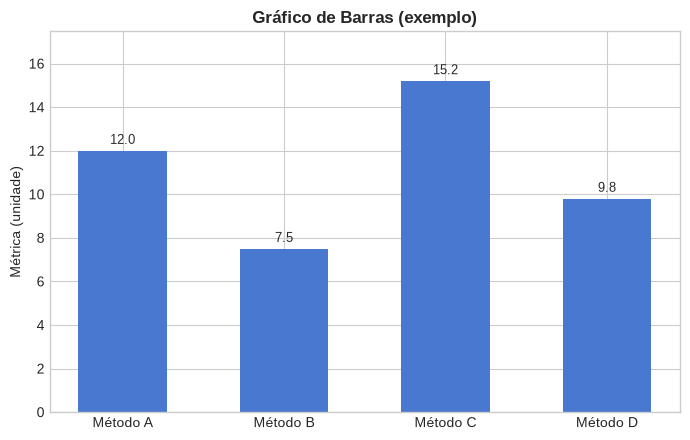
\includegraphics[width=\columnwidth]{results/grafico_barras.png}
	\caption{Legenda do gráfico de barras.}
	\label{fig:grafico-barras}
\end{figure}

\begin{figure}[H]
	\centering
	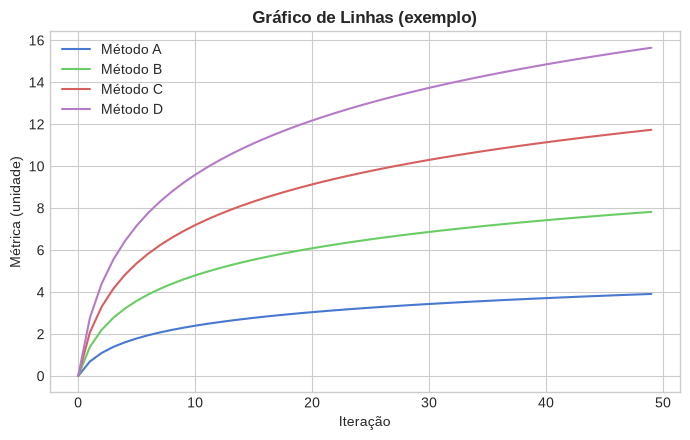
\includegraphics[width=\columnwidth]{results/grafico_linhas.png}
	\caption{Legenda do gráfico de linhas.}
	\label{fig:grafico-linhas}
\end{figure}

\subsection{Discussão}
\label{subsec:discussao}
% Interprete os resultados à luz das propriedades teóricas da
% Seção~\ref{sec:modelagem} em diante: o comportamento observado era
% esperado? Explique discrepâncias e limitações dos experimentos.
\lipsum[18]
